%%%%%%%%%%%%%%%%%%%%%%%%%%%%%%%%%%%%%%%%%%%%%%%%%%%%%%%%%%%%%%%%%%%%%%%%%%%%%%%
% Chapter 3: Resultados
%%%%%%%%%%%%%%%%%%%%%%%%%%%%%%%%%%%%%%%%%%%%%%%%%%%%%%%%%%%%%%%%%%%%%%%%%%%%%%%

%++++++++++++++++++++++++++++++++++++++++++++++++++++++++++++++++++++++++++++++
Este capítulo se centrará en explicar las características que incorpora {\it ghedsh} tras la etapa de desarrollo tratada en el capítulo anterior.
\bigskip

Se hará una distinción entre comandos del núcleo y comandos incorporados ({\it built-in commands}). Los comandos del núcleo, son aquellos que no trabajan con los datos de GitHub del usuario pero que, sin embargo, son
esenciales desde el punto de vista la usabilidad y experiencia de usuario con el CLI.
\bigskip

Por otro lado, los comandos incorporados sí trabajan con los datos de GitHub del usuario identificado. Permiten realizar diversas tareas, priorizando la rapidez en la ejecución de las mismas y la facilidad de uso de la herramienta.

%---------------------------------------------------------------------------------
\section{Autenticación con credenciales de GitHub}
\label{3:sec:1}

El contenido de esta sección pretende explicar el proceso de autenticación que debe seguir el usuario al usar {\it ghedsh} por primera vez.
\bigskip

Dicho proceso es necesario, puesto que se trabajan con los datos que dispone el usuario en GitHub. Además, la API REST v3 requiere, para ciertas consultas (en especial, modificaciones como crear repositorios, equipos y administrar la configuración), verificar la identidad del usuario. Si no fuera así, se podrían llevar a cabo comportamientos indeseados.
\bigskip

En {\it ghedsh}, se realiza la autenticación con {\it OAuth access token}\cite{B16}, que consiste, en una definición muy simplificada, en una cadena de caracteres alfanuméricos que actúa como una contraseña. No obstante,
en este caso de uso es mucho más potente y segura. Las principales ventajas son:
\begin{itemize}
	\item Es revocable, es decir, el {\it token} puede dejar de ser válido, eliminando el acceso para ese {\it token} en particular, sin que el usuario tenga que cambiar su contraseña en todos sus accesos.
	\item Sus permisos son configurables, esto es, un {\it token} puede ser válido sólo para ciertos recursos de una API. De esta manera, se conceden permisos de forma más controlada.
\end{itemize}

Para sintetizar este apartado, el usuario que utilice por primera vez {\it ghedsh}, debe verificar su identidad mediante sus credenciales (nombre de usuario y contraseña) de GitHub y se
generará de forma automática un {\it token} de acceso con los permisos necesarios para usar la herramienta.

\begin{figure}[H]
	\begin{center}
	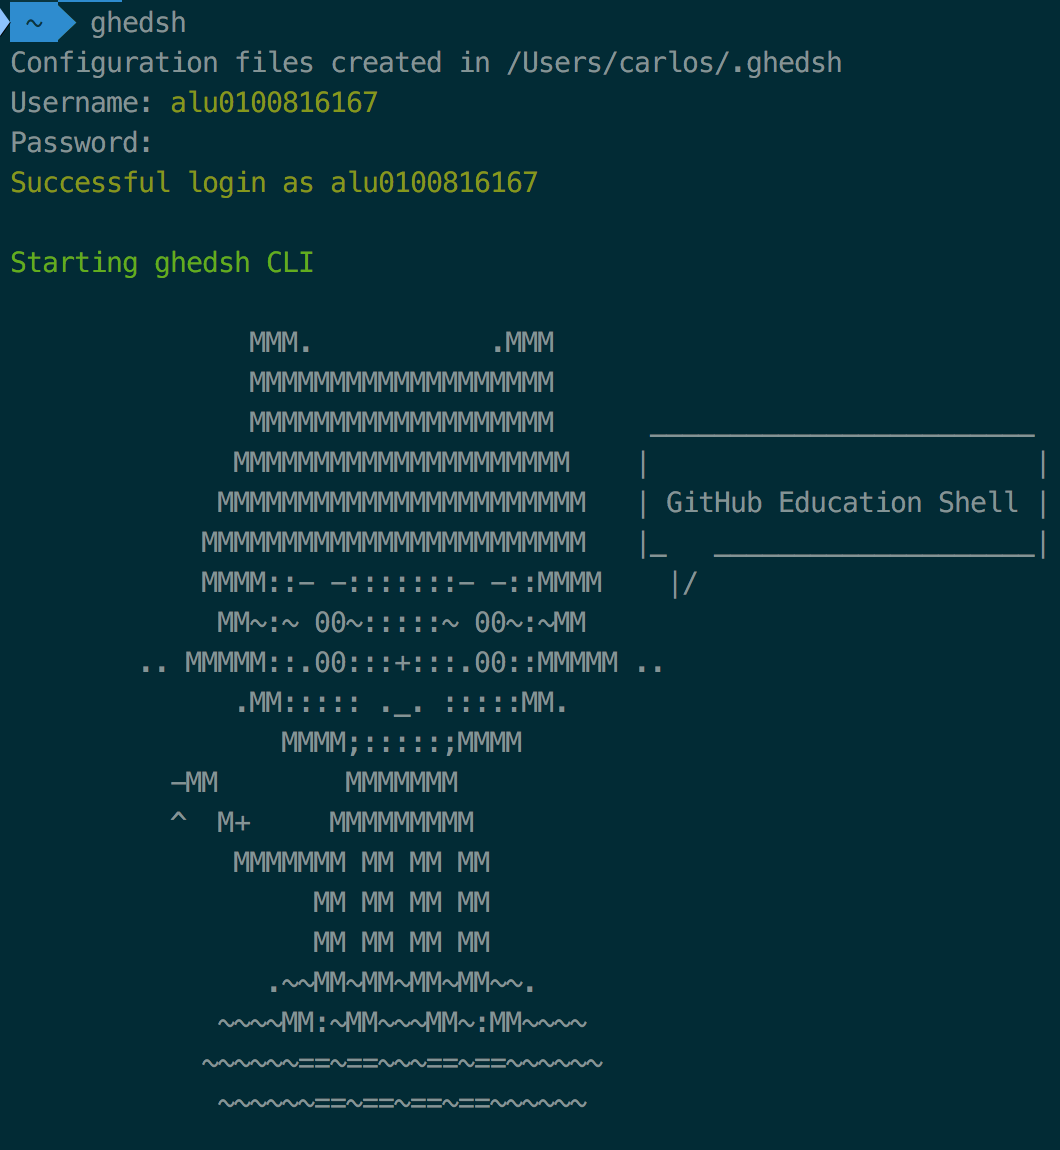
\includegraphics[width=0.45\textwidth]{images/login-example}
	\caption{Ejemplo de autenticación al usar ghedsh por primera vez.}
	\label{fig:masterv1}
	\end{center}
\end{figure}

%------------------------------------------------------------------------------------------------------------
\section{Comandos del núcleo de ghedsh}
\label{3:sec:2}

Como se ha indicado en la introducción de este tercer capítulo, se han separado, por un lado, los comandos del núcleo de {\it ghedsh} y, por otro, los comandos característicos de {\it ghedsh}.
\bigskip

En esta sección, se explicará este primer grupo de comandos, encargado de tareas relacionadas con el sistema operativo y, lo más importante, hacer que la herramienta sea agradable de manejar para el usuario. Además, se revisarán aspectos importantes de su implementación.

\subsection{Change directory: cd}
\label{3.2.1}
Análogamente al comando {\it cd} de la {\it Bash}\cite{B17}, que permite cambiar nuestro directorio actual de trabajo, en {\it ghedsh} también existe este comando. No obstante, aunque la idea es similar, existen diferencias a la hora de usarlo.
\bigskip

En nuestro sistema operativo (tipo Unix)\cite{B18}, cuando realizamos la operación {\it cd}, sólo podemos movernos entre directorios (dependiendo de los permisos). Dado que en {\it ghedsh} no existen directorios como tal, hablaremos de contextos.
Los contextos en esta herramienta hacen referencia a nivel de usuario, nivel de organización, nivel de repositorio, etcétera.
\bigskip

Imaginemos por un momento que nuestro usuario se llama \verb ejemplo , disponemos de un repositorio que se llama \verb ejemplo  y una organización denominada \verb ejemplo . Ésto es totalmente válido, puesto que lo que no permite GitHub es que dos usuarios se llamen igual, que el usuario tenga dos repositorios con el mismo nombre o dos organizaciones bajo el mismo nombre.
Entonces, debemos proporcionar alguna manera de desambiguar a qué contexto nos queremos cambiar.
\bigskip

En {\it ghedsh} se ha optado por el siguiente planteamiento: para realizar la operación de
{\it cd}, es necesario especificar el tipo de contexto (nivel) al que queremos cambiarnos, así, aunque el usuario se encuentre en el caso anteriormente comentado, {\it ghedsh} es capaz de saber a qué contexto debe cambiar.
La sintaxis del comando sería \verb cd  \verb <tipo>  \verb <nombre|Regexp> , donde nombre es la cadena de texto que identifica al tipo, o bien, una expresión regular que mostraría las cadenas que han casado.
\bigskip

Los tipos de contexto que actualmente se soportan en {\it ghedsh} son:
\begin{itemize}
	\item \textbf{Nivel de usuario}: estando a nivel de usuario, éste se puede cambiar a cualquiera de sus repositorios o a cualquier organización a la que pertenezca, como vemos a continuación:
		\begin{itemize}
			\item Repositorio del usuario: \verb cd   \verb repo  \verb <nombre|/Regexp/> .
			\item Organización del usuario: \verb cd   \verb org  \verb <nombre|/Regexp/> .
		\end{itemize}
	\item \textbf{Nivel de organización}: estando a nivel de una organización de la que es miembro el usuario autenticado, ({\it ghedsh} sabrá que se refiere al entorno de la organización a la que se ha cambiado) se puede mover a:
		\begin{itemize}
			\item Repositorio de la organización: \verb cd   \verb repo  \verb <nombre|/Regexp/> .
			\item Equipo de la organización: \verb cd   \verb team  \verb <nombre|/Regexp/> .
		\end{itemize}
\end{itemize}

Además, si deseamos volver al contexto anterior, haremos de la misma manera que en sistemas operativos tipo Unix: \verb cd  \verb ..  . Hay que tener en cuenta que, actualmete, no se puede realizar la operación de volver al contexto anterior y cambiar a otro de manera simultánea (como en Unix \verb cd  \verb ../another/dir  ), es necesario hacerlo por separado.


\subsubsection{Detalles de implementación}
Puesto que se trata de uno de los comandos más importantes de {\it ghedsh}, se comentarán los aspectos destacados de la implementación del mismo, incluyendo las dificultades encontradas.
\bigskip





%------------------------------------------------------------------------------------------------------------
\section{Comandos incorporados en ghedsh}
\label{3:sec:3}   
    

%------------------------------------------------------------------------------------------------------------
\section{Comandos que facilitan el proceso de evaluación}
\label{3:sec:4}  
        	
	
%------------------------------------------------------------------------------------------------------------
\subsection{Automatizar la ejecución de scripts en los repositorios}
\label{subsec:3.1.3} 
	    
    
		
%------------------------------------------------------------------------------------------------------------
\subsection{Recopilar la información obtenida de la automatización de tareas}
\label{subsec:3.1.4}

    Una vez ejecutados los scripts necesarios para evaluar un determinado repositorio, es posible generar un GitBook con el resultado de la ejecución de los mismos. Este libro se genera en formato PDF y en HTML.
\bigskip
    
    En función del contexto dónde nos encontremos dentro de la herramienta, podremos:
    \begin{itemize}
    	\item Crear un GitBook en el repositorio en el que nos encontremos.
    	\item Crear un GitBook en un determinado repositorio.
	    \item Crear un GitBook en todos los repositorios que coincidan con una determinada expresión regular.
	    \item Crear un GitBook en todos los repositorios de una asignación coincidan con una determinada expresión regular.
    \end{itemize}
		
\newpage
%---------------------------------------------------------------------------------
\section{Funcionalidades extra}
\label{3:sec:2}

Además de las funcionales solicitadas en este Trabajo de Fin de Máster, se han añadido una serie de funcionalidades extra que, a pesar de no ser requeridas, brindan al usuario de una mejor experiencia de uso del programa:

\begin{itemize}
  \item Autocompletado de los comandos disponibles en función del contexto donde nos encontremos (nivel principal, organización o repositorio).
	\item Opción de ayuda que muestra la descripción de los comandos y cómo se utilizan. Esta ayuda varía dependiendo del contexto donde nos encontremos.
	\item Opción de visualizar el directorio de trabajo donde se ha ejecutado el programa. Útil para determinar rutas relativas de los scripts que se desean ejecutar.
	\item Opción para conocer el propietario de cada repositorio. En el caso de que el repositorio pertenezca a una organización, mostrará los contribuyentes de ese repositorio.
\end{itemize}

NOTA: se puede consultar toda la información referente a los comandos del programa en el Apéndice 2.

%---------------------------------------------------------------------------------
\section{Problemas encontrados y soluciones}
\label{3:sec:3}

A continuación se detallan los problemas encontrados durante la implementación de la herramienta y las soluciones encontradas para los mismos:

%---------------------------------------------------------------------------------
\subsection{Asincronía}
\label{subsec:3.3.1}

Una de las características más importantes del lenguaje JavaScript es la asincronía. Usa un modelo de operaciones de entrada/salida sin bloqueo y orientado a eventos, que lo hace ligero y eficiente. Sin embargo, algunas acciones que debía realizar esta herramienta debían de ser síncronas. Ejemplos son el login del usuario y ejecución de scripts.
\bigskip

{\normalsize {\bfseries Solución}}
\bigskip

La solución a este comportamiento pasó por realizar un amplio estudio de la documentación para usar mecanismos que permitieran bloquear la ejecución de la herramienta en las partes que deseábamos. Los mecanismos usados han sido:

\begin{itemize}
	\item Funciones síncronas del propio lenguaje.
	\item Promesas
	\item Métodos async/await
	\item Librerías con métodos implementados de manera síncrona.
\end{itemize}

%---------------------------------------------------------------------------------
\subsection{Autocompletado de comandos}
\label{subsec:3.3.2}

Para el manejo de los flujos de lectura y escritura de la herramienta, se ha utilizado la interfaz nativa de Node.js (Readline). Esta interfaz provee de una función de autocompletado para el texto que escribe el usuario.

Sin embargo, sólo funciona con la primera palabra (comando) que escribe. Tras investigar al respecto y buscar posibles librerías alternativas, no existía ninguna solución que corrigiera este comportamiento.
\bigskip

{\normalsize {\bfseries Solución}}
\bigskip

Realizando numerosas pruebas, se halló una manera propia de conseguir completar más de un comando en la misma línea. Cuando realice los test de aceptación pertinentes requeridos por la comunidad de Node, solicitaré un Pull Request a su repositorio con esta mejora.


%---------------------------------------------------------------------------------
\section{Perfil del usuario de ghshell}
\label{3:sec:4}

El uso de \verb|ghshell| está especialmente dirigido a un determinado grupo de profesores: nos referimos al perfil de un profesor, principalmente docente en alguna rama de Ingeniería, con conocimientos avanzados en programación y en herramientas de control de versiones.

No obstante, ya que la curva de aprendizaje de \verb|ghshell| no es excesiva y dado que el uso de las herramientas de control de versiones no se limita exclusivamente a repositorios de código fuente, se puede extender su uso para el resto de profesorado y usuarios con otros roles. Basta con tener claras unas nociones básicas de informática, junto con la lectura y asimilación previa de la documentación de la herramienta.
